\documentclass[hyperref]{ctexart}
\usepackage[left=2.50cm, right=2.50cm, top=2.50cm, bottom=2.50cm]{geometry} %页边距
\usepackage{helvet}
\usepackage{amsmath, amsfonts, amssymb} % 数学公式、符号
\usepackage[english]{babel}
\usepackage{graphicx}   % 图片
\usepackage{url}        % 超链接
\usepackage{bm}         % 加粗方程字体
\usepackage{multirow}
\usepackage{booktabs}
\usepackage{algorithm}
\usepackage{algorithmic}
\usepackage{fancyhdr} %设置页眉、页脚
\pagestyle{fancy}
\lhead{}
\chead{}
\lfoot{}
\cfoot{}
\rfoot{}
\usepackage{hyperref} %bookmarks
\hypersetup{colorlinks, bookmarks, unicode} %unicode
\usepackage{multicol}
\title{\textbf{法拉第效应}}
\author{\sffamily 赵宇航}
\date{}
\begin{document}
\maketitle
%\indent{\bf 摘要: }\\	
%\begin{multicols}{2}
\CTEXsetup[format={\Large\bfseries}]{section}
	\section{实验简介}
	1845年,法拉第(M.Faraday)在探索电磁现象和光学现象之间的联系时,发现了一种现象:当一束平面偏振光穿过介质时,如果在介质中,沿光的传播方向上加上一个磁场,就会观察到光经过样品后偏振面转过一个角度,即磁场使介质具有了旋光性,这种现象后来就称为法拉第效应。法拉第效应第一次显示了光和电磁现象之间的联系,促进了对光本性的研究。之后维尔德(Verdet)对许多介质的磁致旋光进行了研究,发现了法拉第效应在固体、液体和气体中都存在。

	法拉第效应有许多重要的应用,尤其在激光技术发展后,其应用价值越来越受到重视。如用于光纤通讯中的磁光隔离器,是应用法拉第效应中偏振面的旋转只取决于磁场的方向,而与光的传播方向无关,这样使光沿规定的方向通过同时阻挡反方向传播的光,从而减少光纤中器件表面反射光对光源的干扰;磁光隔离器也被广泛应用于激光多级放大和高分辨率的激光光谱,激光选模等技术中。在磁场测量方面,利用法拉第效应驰豫时间短的特点制成的磁光效应磁强计可以测量脉冲强磁场、交变强磁场。在电流测量方面,利用电流的磁效应和光纤材料的法拉第效应,可以测量几千安培的大电流和几兆伏的高压电流。

	磁光调制主要应用于光偏振微小旋转角的测量技术,它是通过测量光束经过某种物质时偏振面的旋转角度来测量物质的活性,这种测量旋光的技术在科学研究、工业和医疗中有广泛的用途,在生物和化学领域以及新兴的生命科学领域中也是重要的测量手段。如物质的纯度控制、糖分测定;不对称合成化合物的纯度测定;制药业中的产物分析和纯度检测;医疗和生化中酶作用的研究;生命科学中研究核糖和核酸以及生命物质中左旋氨基酸的测量;人体血液中或尿液中糖份的测定等。在工业上,光偏振的测量技术可以实现物质的在线测量;在磁光物质的研制方面,光偏振旋转角的测量技术也有很重要的应用。

	本实验的目的是学习法拉第磁致旋光效应的基本原理,学习利用消光法测量旋光角并测量几种不同材料的维尔德常数。
	\section{实验原理}
	\subsection{法拉第效应}
	实验表明,在磁场不是非常强时,如图1所示,偏振面旋转的角度$\theta$与光波在介质中走过的路程L及介质中的磁感应强度在光的传播方向上的分量B成正比,即:
	\begin{equation}
	\theta=VBL
	\end{equation}

	比例系数V由物质和工作波长决定,表征着物质的磁光特性,这个系数称为维尔德(Verdet)常数。
	\begin{center}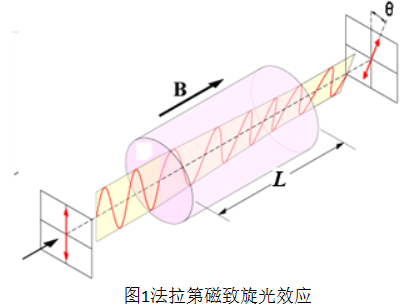
\includegraphics[scale=0.4]{t1}\end{center}

	维尔德常数V与磁光材料的性质有关,对于顺磁、弱磁和抗磁性材料(如重火石玻璃等),V为常数,即$\theta$与磁场强度B有线性关系;而对铁磁性或亚铁磁性材料(如YIG等立方晶体材料),$\theta$与B不是简单的线性关系。表1为几种物质的维尔德常数。几乎所有物质(包括气体、液体、固体)都存在法拉第效应,不过一般都不显著。
	\begin{center}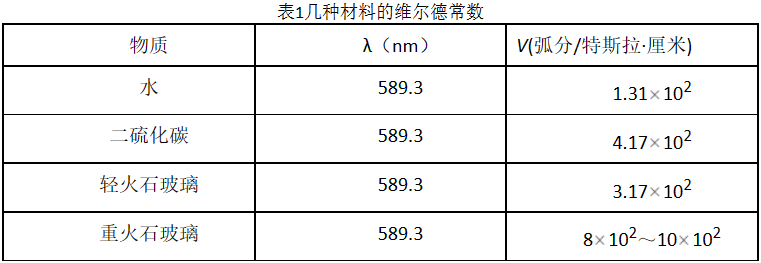
\includegraphics[scale=0.4]{b1}\end{center}

	对于每一种给定的物质,法拉第旋转方向仅由磁场方向决定,而与光的传播方向无关(不管传播方向与磁场同向或者反向),这是法拉第磁光效应与某些物质的固有旋光效应的重要区别。固有旋光效应的旋光方向与光的传播方向有关,即随着顺光线和逆光线的方向观察,线偏振光的偏振面的旋转方向是相反的,因此当光线往返两次穿过固有旋光物质时,线偏振光的偏振面没有旋转。而法拉第效应则不然,在磁场方向不变的情况下,光线往返穿过磁致旋光物质时,法拉第旋转角将加倍。利用这一特性,可以使光线在介质中往返数次,从而使旋转角度加大。这一性质使得磁光晶体在激光技术、光纤通信技术中获得重要应用。
	\begin{center}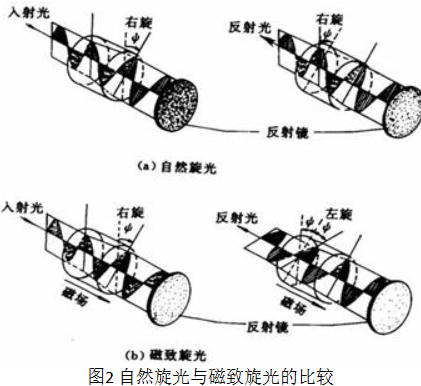
\includegraphics[scale=0.4]{t2}\end{center}

	与固有旋光效应类似,法拉第效应也有旋光色散,即维尔德常数随波长而变,一束白色的线偏振光穿过磁致旋光介质,则紫光的偏振面要比红光的偏振面转过的角度大,这就是旋光色散。实验表明,磁致旋光物质的维尔德常数V随波长$\lambda$的增加而减小(如图3),旋光色散曲线又称为法拉第旋转谱。
	\begin{center}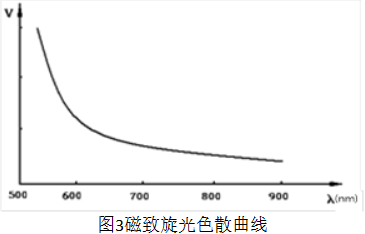
\includegraphics[scale=0.4]{t3}\end{center}

	根据电磁波与物质相互作用的理论,物质的维尔德常数V由如下公式决定
	\begin{equation}
	V=\frac{e}{2mc}\lambda \frac{dn}{d\lambda}
	\end{equation}

	式中e/m为电子的荷质比,c为真空中光速,$\lambda$为光波长,n为折射率,dn/d$\lambda$为介质的色散。如果介质色散满足柯西公式n=a+b/$\lambda^2$(a和b为介质的色散常数),则将柯西公式代入公式(2)得到V=eb/(mc$\lambda^2$),此时,维尔德常数正比于1/$\lambda^2$。电子的荷质比e/m 可以根据纯光学测量和已知光速计算得到。在一些物质中用这种方法得到的e/m值和理论值符合的很好,说明在这些物质中,法拉第效应是由于电子的本征振动引起的。

	上式中,左旋和右旋只是相对于磁场方向而言的,与光波的传播方向同磁场方向相同或相反无关。因此,法拉第效应便有与自然旋光现象完全不同的不可逆性。

	\subsection{磁光调制原理}
	根据马吕斯定律,如果不计光损耗,则通过起偏器,经检偏器输出的光强为
	\begin{equation}
	I=I_0 cos^2 \alpha
	\end{equation}

	式中,$I_0$为起偏器同检偏器的透光轴之间夹角$\alpha=0$或$\alpha=\pi$时的输出光强。若在两个偏振器之间加一个由励磁线圈(调制线圈)、磁光调制晶体和低频信号源组成的低频调制器(参见图4),则调制励磁线圈所产生的正弦交变磁场$B=B_0sin \omega t$,能够使磁光调制晶体产生交变的振动面转角$q=q_0sin \omega t$,q0称为调制角幅度。此时输出光强由式(3)变为
	\begin{equation}
	I =I_0 cos^2 (\alpha+\theta)=I_0 cos^2 (\alpha+\theta_0 sin \omega t)
	\end{equation}

	由式(4)可知,当$\alpha$一定时,输出光强I仅随q变化,因为q是受交变磁场B或信号电流$i=i_0sin \omega t$控制的,从而使信号电流产生的光振动面旋转,转化为光的强度调制,这就是磁光调制的基本原理。
	\begin{center}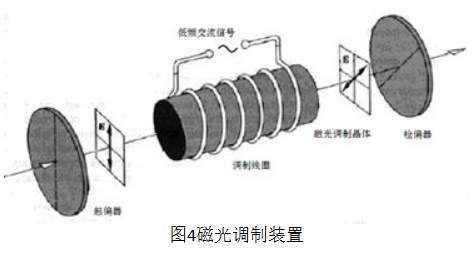
\includegraphics[scale=0.4]{t4}\end{center}

	\section{实验内容}
	1. 测量励磁电流恒定的条件下,线圈的磁感应强度;并以I为横坐标,为纵坐标,作出~I的拟合曲线,求出曲线的斜率。

	选择合适的励磁电流(I=0A,0.25A,0.5A,0.75A,1.0A)用特斯拉计反复测量线圈两端管口的磁感应强度,线圈内部的磁感应强度B近似满足关系1.8B管口,由此求得线圈内部的磁感应强度。

	2. 线圈中恒定磁场条件下,测量不同波长激光的重火石玻璃的维尔德常数。

	将激光器,起偏器,螺旋线圈,检偏器和白屏按顺序依次摆放好,打开激光器调整起偏器和检偏器夹角为 90度此时屏幕上光斑消失。然后接通电源,选择合适的励磁电流(I=±0.5A,±1A),线圈中放入重火石玻璃样品,重新调至消光,记录磁致旋光的角度,从而计算重火石玻璃的维尔德常数

	3. 测量液体的维尔德常数

	将线圈中的样品换成纯水、乙醇或者食盐水,重复 2 的操作,测量并计算液体的维尔德常数。

	4. 磁光调制和解调。

	调制:打开405nm激光器,将重火石玻璃放入线圈,信号发生器输入波形接入线圈,其中波形选择为正弦,频率为1KHz,幅值为20V。

	解调:将信号发生器频率设置为1KHz,同时将它输入到示波器的CH1通道。其中,光敏电阻与取样电阻R串联接入15V直流电压,取样电阻为90KΩ,将示波器并联在取样电阻两端接入CH2。在消光位置附近转动检偏器,观察并记录CH2的频率的变化并分析原因(可观察李萨如图)。

	\section{实验结果}
	\section{讨论}













%\end{multicols}
\end{document}